\chapter{Modello Progettuale}
	\label{cap:modelloprogettuale}

\section{Architettura}
Il diagramma del sistema da implementare pu\`o essere 
rappresentato semplicemente come in figura \ref{fig:architettura}
\begin{figure}[H]
	\centering
	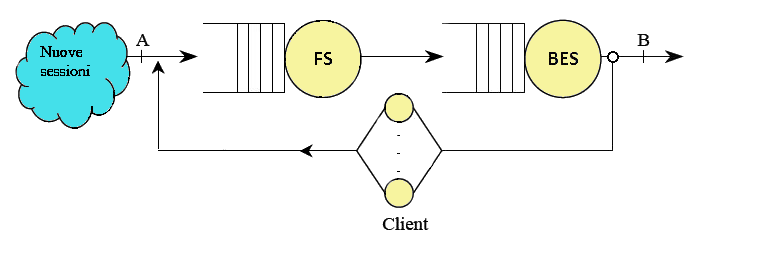
\includegraphics[scale=0.7]{img/architettura.png}
	\caption[Architettura del sistema]{Rappresentazione grafica 
dell'architettura del sistema.}
	\label{fig:architettura}
	\end{figure}
All'inizio della simulazione il primo evento che si verifica \'e sempre l'arrivo 
di una nuova sessione (evento NewSession).

\vspace{0.5cm}I client del centro delle sessioni attive, all'interno del ramo di 
retroazione sono paralleli ed infiniti, definendo un infinity server.

\vspace{0.5cm}I nuovi eventi in arrivo verso il sistema verranno 
posti in coda al FrontServer, nel caso in cui non possano essere serviti. Come 
\'e visibile dalla figura precedente, la sessione una volta servita dal 
Front Server verr\`a posta in coda verso il Back-End Server finch\'e non verr\`a 
servita da quest'ultimo. Infine le sessioni saranno completate oppure poste 
nella zona di "\textit{Thinking}" finch\'e non verranno reinserite nella coda 
del Front-End in attesa di essere serviti, passando attraverso un ramo di 
feedback.
 
\section{Clock di simulazione e schedulazione di  Eventi}
Nella fase implementativa si tiene conto dell'avanzamento del tempo per mezzo 
della variabile \textit{current\_time}. Il meccanismo di avanzamento del tempo 
scelto \'e il \textit{Next-Event Time Advance}. Questa scelta garantisce che gli 
eventi occorrano nella sequenza corretta, ovvero vengono processati in ordine 
crescente rispetto al tempo di schedulazione. Si utilizza, inoltre, il flag di 
\textit{arrivals} per regolare l'accettazione delle nuove sessioni, necessaria per il meccanismo di overload management: se impostata 
a zero vengono inibiti i nuovi arrivi\footnote{Ovvero viene eseguito il drop 
della sessione in entrata o l'abort se la sessione \'e gi\`a nel sistema}, 
altrimenti si procede normalmente con la simulazione.

\section{Event List}
Per la gestione degli eventi si utilizza una lista collegata di strutture 
\textit{Event}, come quella mostrata in figura, salvate in ordine crescente 
rispetto al tempo. Ogni nodo contiene il tempo di occorrenza e la sua tipologia. 
Un gestore di eventi \'e utilizzato per il demultiplexing di tale lista facendo 
uso di una funzione pop() per ottenere il \textit{Next-Event} da processare.
\begin{figure}[H]
  \centering
  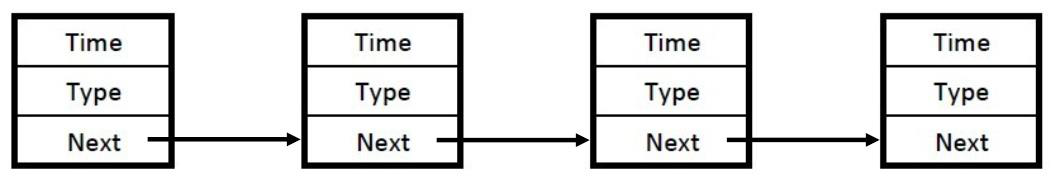
\includegraphics[scale=0.5]{img/EventList.png}
  \caption[EventList]{Struttura lista eventi}
  \label{fig:eventList}
\end{figure}

\section{Arrival Queue}
Al fine di ottenere informazioni riguardo i tempi di attesa che le sessioni 
sperimentano durante la loro permanenza nel sistema, si utilizzano delle 
strutture dati atte a registrare tali informazioni ed utilizzate negli algoritmi 
del calcolo delle medie. Tali strutture, denominate \textit{ArrivalQueue}, 
immagazzinano i tempi di arrivo delle sessioni nelle sottosezioni del sistema 
(ovvero quando una sessione entra nel \textit{Front Server} o nella sua coda, 
quando entra nel \textit{Back-End Server}, e cos\`i via). Ad ogni completamento 
sperimentato da una sessione viene utilizzata la coda relativa e si calcola, per 
differenza, il tempo effettivo che la sessione ha passato in quella parte di 
sistema. Tutto ci\`o \'e possibile grazie all'ipotesi che l'ordine di arrivo, 
all'interno delle code del sistema, \'e sempre \texttt{preservato}. Infatti la 
prima sessione ad entrare nella coda del Front Server, ad esempio, sar\`a la 
prima a lasciarlo.

\section{Request Queue}
Dal momento che \'e impossibile identificare una singola richiesta utilizzando 
la Next-Event Simulation, il problema di preservare l'informazione riguardante 
il numero di richieste attive di cui si compone una sessione viene risolto con 
la struttura dati \textit{Request Queue}. 

Ad ogni richiesta completata si decrementa il contatore delle richieste relative 
a quella sessione in modo da propagare tale informazione a tutte le richieste 
future. Quando il contatore arriva a zero la sessione viene completata del tutto 
e di conseguenza abbandona il sistema.

\section{Client Order List}
Per preservare una Next-Event Simulation priva di contaminazioni derivanti dall'
aggiunta di dati identificanti le sessione o le richieste all'interno degli eventi di base, 
la Client Order List permette di conservare le 
informazioni relative all'ordine di arrivo e di uscita degli utenti all'interno 
del centro Client. Attraverso questa informazione \'e possibile gestire il 
corretto ordine degli elementi della Request Queue nonostante siano condizionati 
da una mancanza di determinismo circa l'ordine di completamento degli utenti 
durante il loro periodo di Think Time.


\section{Personalizzazione del modello}
In base alle scelte effettuate dall'utente nella fase di \textit{setup} \'e 
possibile decidere di avviare la simulazione:
\begin{itemize}
\item senza \textbf{Overload Management}
\item con \textbf{Overload Management}
\end{itemize}
 
\noindent \'E inoltre possibile scegliere quale distribuzione utilizzare tra:
\begin{itemize}
\item \textit{Esponenziale}
\item \textit{10-Erlang}
\item \textit{Iperesponenziale}
\end{itemize}

\noindent Infinie si devono impostare i parametri riguardanti il \textit{numero di batch}
e la \textit{grandezza del batch} stesso.

%%Diagrammi per spiegazioni
\section{Algoritmi di Gestioni eventi}
\subsection{NewSession}
\begin{figure}[H]
  \centering
  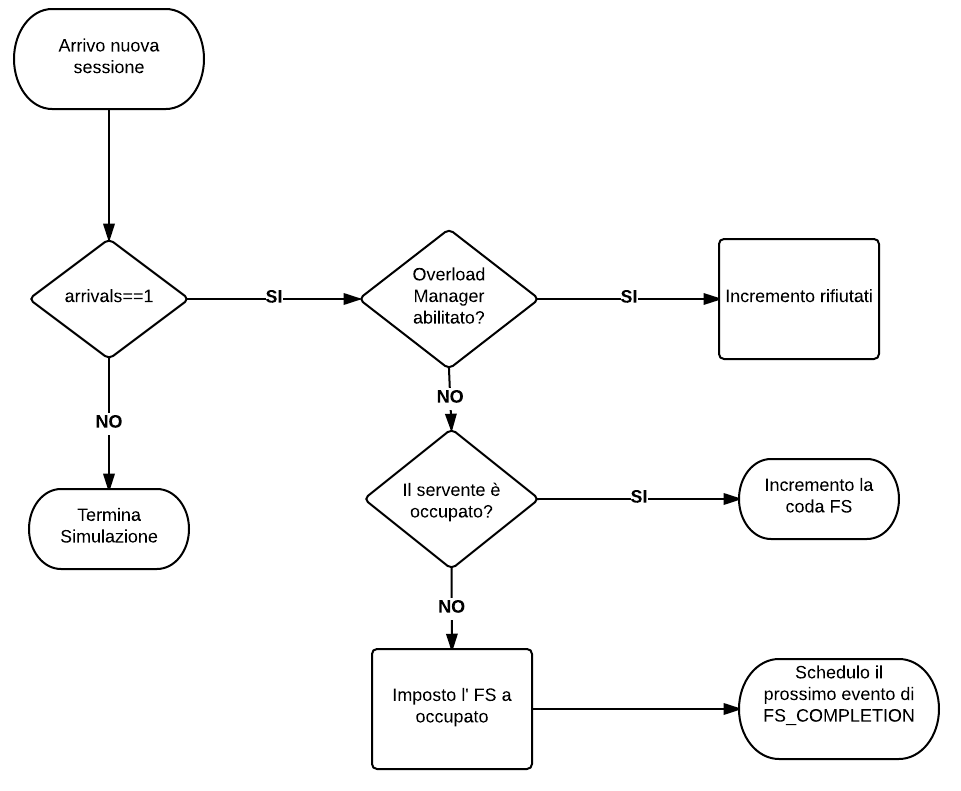
\includegraphics[scale=0.35]{img/NewSession.png}
  %\caption[NewSession]{Struttura lista eventi}
  \label{fig:NewSession}
\end{figure}
\subsection{FS Completion}
\begin{figure}[H]
  \centering
  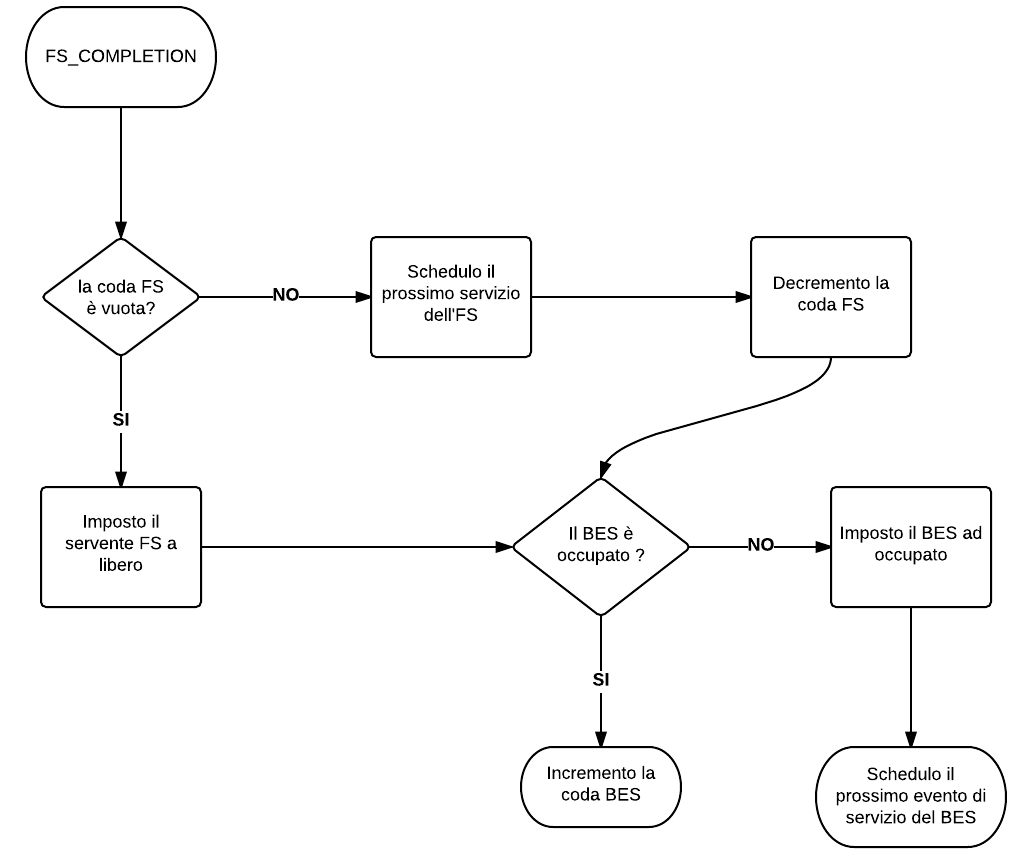
\includegraphics[scale=0.35]{img/FS_Completion.png}
  %\caption[NewSession]{Struttura lista eventi}
  \label{fig:FS_Completion}
\end{figure}

\subsection{BES Completion}
\begin{figure}[H]
  \centering
  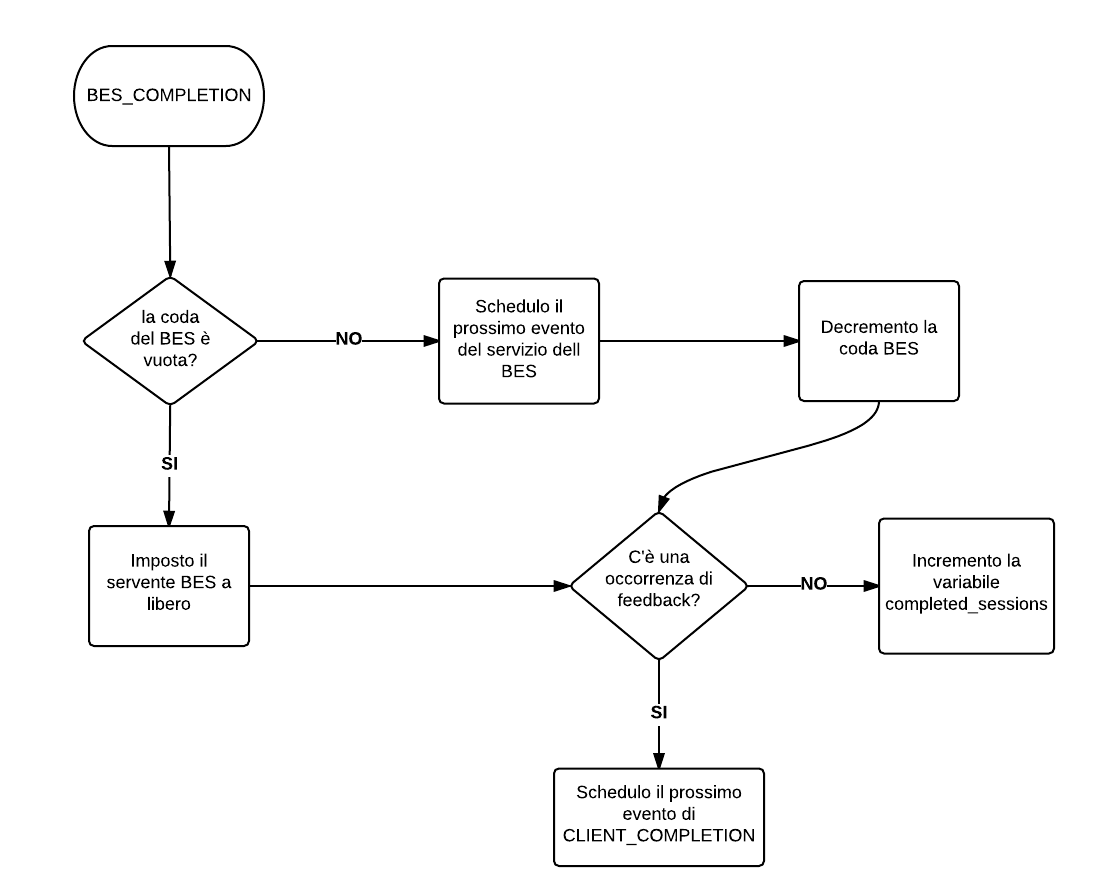
\includegraphics[scale=0.40]{img/BES_Completion.png}
  %\caption[NewSession]{Struttura lista eventi}
  \label{fig:FS_Completion}
\end{figure}

\subsection{Client Completion}
\begin{figure}[H]
  \centering
  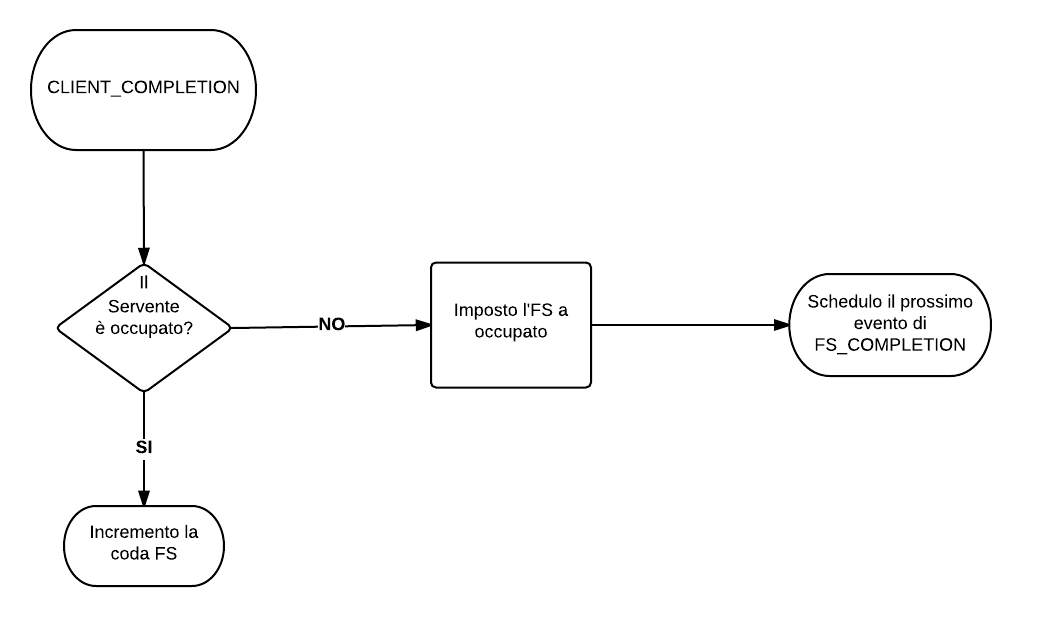
\includegraphics[scale=0.45]{img/CLIENT_Completion.png}
  %\caption[NewSession]{Struttura lista eventi}
  \label{fig:FS_Completion}
\end{figure}

\section{Indici di prestazioni}
Il simulatore qui utilizzato genera un insieme di statistiche che permettono di ricavare 
informazioni utili per comprendere il comportamento del sistema.
\vspace{0.5cm}
\noindent Gli indici di prestazione calcolati sono:
\begin{itemize}
\item \textbf{Useful Troughput}:
indica il totale delle sessioni completate nell'unit\`a di tempo. 
Tale indice viene calcolato attraverso il rapporto tra le sessioni totali 
processate dal sistema e l'intervallo di tempo necessario per ultimare questo 
compito. Il troughput basato sulle sessioni \'e un ottimo indice per valutare 
il numero di utenti serviti dal sistema in un intervallo dato, risultando una 
misura sensibile per l'utente finale.

\item \textbf{Tempo di Risposta del Sistema}:
viene inteso come la somma del tempo di risposta: Tempo in coda + Tempo di 
Servizio.
In pratica il tempo di risposta \'e inteso come il tempo che intercorre tra l'istante in cui una
richiesta entra nel Front Server e l'uscita della stessa dal Back-End Server.

\item \textbf{Drop Ratio}:
misura il rapporto tra il totale delle sessioni rifiutate dal sistema ed il 
numero di sessioni totali che tentano di entrare nel sistema (accettate + 
rifiutate).

\item \textbf{Abort Ratio}:
\'e il rapporto tra le richieste abortite ed il totale di richieste processate 
dal sistema.
Questo \'e dovuto al fatto che una richiesta pu\`o rientrare nel sistema, 
tuttavia in condizioni di saturazione, tale richiesta non \`e in grado di poter 
rientrare all'interno del Front Server, quindi viene appunto abortita.

\end{itemize}
